% chktex-file 1
% chktex-file 2
% chktex-file 3
% chktex-file 8
% chktex-file 9
% chktex-file 12
% chktex-file 13
% chktex-file 16
% chktex-file 18
% chktex-file 24
% chktex-file 26
% chktex-file 35
% chktex-file 44
% chktex-file 45

\documentclass[]{article}
\usepackage[utf8]{inputenc}
\usepackage[english]{babel}

\usepackage[]{csvsimple}
\usepackage{float}

\usepackage{ragged2e}
\usepackage[left=25mm, right=25mm, top=15mm]{geometry}
\geometry{a4paper}
\usepackage{graphicx}
\usepackage{booktabs}
\usepackage{paralist}
\usepackage{subfig} 
\usepackage{fancyhdr}
\usepackage{amsmath}
\usepackage{amssymb}
\usepackage{amsfonts}
\usepackage{amsthm}
\usepackage{mathtools}
\usepackage{enumitem}
\usepackage{titlesec}
\usepackage{braket}
\usepackage{gensymb}
\usepackage{url}
\usepackage{hyperref}
\usepackage{csquotes}
\usepackage{multicol}
\usepackage{graphicx}
\usepackage{wrapfig}
\usepackage{babel}
\usepackage{caption}
\captionsetup{font=small}
\pagestyle{fancy}
\renewcommand{\headrulewidth}{0pt}
\lhead{}\chead{}\rhead{}
\lfoot{}\cfoot{\thepage}\rfoot{}
\usepackage{sectsty}
\usepackage[nottoc,notlof,notlot]{tocbibind}
\usepackage[titles,subfigure]{tocloft}
\renewcommand{\cftsecfont}{\rmfamily\mdseries\upshape}
\renewcommand{\cftsecpagefont}{\rmfamily\mdseries\upshape}

\let\oldsection\section% Store \section
\renewcommand{\section}{% Update \section
	\renewcommand{\theequation}{\thesection.\arabic{equation}}% Update equation number
	\oldsection}% Regular \section
\let\oldsubsection\subsection% Store \subsection
\renewcommand{\subsection}{% Update \subsection
	\renewcommand{\theequation}{\thesubsection.\arabic{equation}}% Update equation number
	\oldsubsection}% Regular \subsection

\newcommand{\abs}[1]{\left\lvert#1\right\rvert}
\newcommand{\norm}[1]{\left\lVert#1\right\rVert}

\newcommand{\g}{\text{g}}
\newcommand{\m}{\text{m}}
\newcommand{\cm}{\text{cm}}
\newcommand{\mm}{\text{mm}}
\newcommand{\s}{\text{s}}
\newcommand{\N}{\text{N}}
\newcommand{\Hz}{\text{Hz}}

\newcommand{\virgolette}[1]{``\text{#1}"}
\newcommand{\tildetext}{\raise.17ex\hbox{$\scriptstyle\mathtt{\sim}$}}


\renewcommand{\arraystretch}{1.2}

\addto\captionsenglish{\renewcommand{\figurename}{Fig.}}
\addto\captionsenglish{\renewcommand{\tablename}{Tab.}}

\DeclareCaptionLabelFormat{andtable}{#1~#2  \&  \tablename~\thetable}


\title{%
    \Huge Misura del rapporto carica/massa di un elettrone non relativistico \\
    \Large Laboratorio di Ottica, Elettronica e Fisica Moderna \\ C.d.L. in Fisica, a.a. 2023-2024 \\ Università degli Studi di Milano}
\author{\LARGE Lucrezia Bioni, Leonardo Cerasi, Giulia Federica Bianca Coppi \\ Matricole: 13655A, 11410A, 11823A}
\date{2 novembre 2023}

\begin{document}

    \maketitle

    \section{Introduzione}

    \subsection{Scopo}

    L'elettrone è una particella carica e massiva: in questa esperienza ci si propone di misurare il suo rapporto carica-massa $ \frac{e}{m} $ in condizioni non relativistiche. \\
    Le misurazioni vengono effettuate in tre casi distinti: perpendicolarmente, parallelamente e antiparallelamente al campo magnetico terrestre.


    \subsection{Metodo}
    In un'ampolla contenente gas idrogeno a bassa pressione (circa $ 10^{-2}\, \text{torr} $), è posta una resistenza che, essendo percorsa da corrente elettrica alternata, scalda un catodo che emette elettroni per effetto termoelettrico. Questi, accelerati dalla differenza di potenziale $\Delta V$ presente tra il catodo e l'anodo, vengono fatti collimare in un unico fascio, la cui traiettoria viene deviata dalla forza di Lorentz. Quest'ultima, ortogonale al vettore velocità degli elettroni, è generata dal campo magnetico $ B_z $, prodotto dalle bobine di Helmholz poste ai lati dell'ampolla: il cammino percorso dal fascio assume una forma circolare grazie alla regolazione dell'intensità di $B_z$. \\
    Lungo il loro cammino, gli elettroni collidono con le molecole di idrogeno, emettendo fotoni ad una lunghezza d'onda di circa $4500 \text{Å}$.
    Il raggio della circonferenza visibile risulta fondamentale per la determinazione della grandezza interessata, come mostrato dalla seguente equazione:

    \begin{equation}
        \label{e_m}
        \frac{e}{m} = \frac{2 \Delta V}{(B_z R)^2}
    \end{equation}
    dove $ e $ ed $ m $ rappresentano rispettivamente la carica elettrica e la massa dell'elettrone, $\Delta V$ rapprensenta la differenza di potenziale, $B_z$ rappresenta il campo magnetico generato dalle bobine di Helmholz e $ R $ rapprensenta il raggio della circonferezza compiuta dagli elettroni. \\

    In base alla differente influenza del campo magnetico terrestre, il campo magnetico effettivo a cui è sottoposto il fascio di elettroni varia: è dunque necessario andare a stimare il contributo di quest'ultimo in modo da poter fornire un risultato più accurato al valore finale della grandezza interessata.

    \section{Misure}

    \subsection{Per la determinazione del campo magnetico generato dalle bobine di Helmholtz}

    La determinazione delle grandezze utili a fornire un valore di $e/m$ richiede la stima preliminare del raggio medio delle bobine di Helmholz: tale misurazione viene compiuta attraverso l'utilizzo di un calibro di risoluzione $0.02 \text{mm}$. Le bobine di Helmholz hanno la caratteristica di essere poste a una distanza equivalente al loro raggio medio. Pertanto, si procede misurando la loro distanza per eccesso e per difetto - 5 misurazioni per entrambe le distanze - e come valore finale si fornisce la media delle due medie ottenute dai due set di dati. Le misure effettuate sono riportate in Tab. ~\ref{Raggio_bobine} e ~\ref{media_devst_Rb}. Come incertezza, invece, si attribuisce la somma in quadratura delle deviazioni standard dei due set di dati, poiché tale valore è superiore alla risoluzione dello strumento.


    \begin{table}[H]
        \centering
    
        \begin{tabular}{||c|c||}
            \hline
            $R_b \, \text{per difetto\,} \text{[cm]} $ & $R_b \, \text{per eccesso\,} \text{[cm]} $\\
            \hline\hline
    
            $ 13.45 $ & $ 17.77 $ \\\hline
            $ 13.51 $ & $ 17.80 $ \\\hline
            $ 13.48 $ & $ 17.69 $ \\\hline
            $ 13.76 $ & $ 17.74 $ \\\hline
            $ 13.43 $ & $ 17.70 $ \\\hline
        
        \end{tabular}
        \caption{Misure del raggio medio delle bobine di Helmholz per difetto e per eccesso.}
        \label{Raggio_bobine}
    \end{table}
    
    \begin{table}[H]
        \centering
    
        \begin{tabular} {||c|c||c|c||}
            \hline
            $ \text{media per difetto\,} [\text{cm}] $ & $\sigma_{dif} [\text{cm}] $ & $ \text{media per eccesso} [\text{cm}] $ & $\sigma_{ecc} [\text{cm}] $\\
            \hline \hline
    
            $ 13.52 $ & $ 0.14 $ & $ 17.74 $ & $ 0.05 $ \\\hline
    
        \end{tabular}
        \caption{Medie per difetto e per eccesso delle misure del raggio medio delle bobine di Helmholz con relative deviazioni standard}
        \label{media_devst_Rb}
    
    \end{table}
    Il valore finale attribuito al raggio delle bobine di Helmholtz risulta dunque essere:

    \begin{equation}
        \label{misura_Rb}
        R_b = (15.63 \pm 0.07) \, \text{cm}
    \end{equation} 
    Dopo aver determinato, mediante ago magnetico, la direzione della componente orizzontale del campo magnetico terrestre, si orienta l'asse delle bobine ortogonale a tale direzione. Al variare della differenza di potenziale $\Delta V $ tra catodo e anodo e dell'intensità di corrente $I$ che alimenta le bobine di Helmholtz, si misura, attraverso un calibro digitale di risoluzione $\sigma_{D}= 0.01 \text{mm}$, il diametro $D$ della circonferenza percorsa dagli elettroni, da cui si ottiene il valore del raggio $R$ della medesima. L'incertezza a tali misure del raggio ($\sigma_{R}$) è stata attribuita mediante propagazione dell'incertezza sul diametro, stimata pari alla risoluzione del calibro adoperato: 
    \begin{equation}
        \label{sigma_raggioCirc}
        \sigma_{R} = \frac{\sigma_{D}}{\sqrt{2} }
    \end{equation}
    I valori di differenza di potenziale e intensità di corrente, invece, sono stati misurati attraverso un multimetro digitale in modalità, rispettivamente, di Voltmetro (con risoluzione di $0.1 \text{V}$) e di Amperometro (con risoluzione di $0.001 \text{A}$). In entrambi i casi è stata attribuita come incertezza la risoluzione dello strumento, poiché risultava sempre superiore all'intervallo di stabilizzazione del generatore ($\pm 0.1 \%$). Tale set di misure è riportato in Tab. \ref{CM_ortogonale}. \\
    
    Si è ripetuto il medesimo set di misure orientando l'asse delle bobine in direzione parallela (Tab. \ref{CM_parallelo}) e antiparallela (Tab. \ref{CM_antiparallelo}) rispetto alla componente orizzontale del campo magnetico terrestre.

    \subsection{Per la determinzione del campo magnetico terrestre}
    Nelle condizioni in cui la strumentazione viene posta parallelela e antiparallela al campo magnetico terrestre, questo influisce sull'effettivo campo magnetico a cui sono sottoposti gli elettroni lungo la loro orbita: risulta, dunque, necessario dare un valore a questa grandezza in modo da poter correggere le errate stime del rapporto $e/m$. In mezzo ad una coppia di bobine di geometria nota è posto un ago magnetico, che viene fatto deflettere di angoli noti facendo variare l'intensità di corrente che alimenta le bobine (generatrici del campo magnetico). L'intensità di corrente viene misurata mediante multimetro in modalità di Amperometro, con risoluzione di $0.001 \text{A}$ (attribuita come incertezza della misura, poiché maggiore all'intervallo di stabilizzazione del generatore $\pm 0.1 \%$). L'angolo di deflessione, invece, viene misurato con un goniometro, solidale alle bobine, orientato in modo che, a corrente nulla, l'ago magnetico risulti diretto nella direzione $0-180 \degree $ di esso. Come incertezza a tali misure viene attribuita la risoluzione dello strumento: $1 \degree$. Tali misure sono state prese facendo deflettere l'ago magnetico sia in senso orario sia in senso antiorario, e sono riportate in Tabb. \ref{campomagneticoterrestre_sensoorario} , \ref{campomagneticoterrestre_sensoantiorario}.
    

    \section {Analisi Dati}

    \subsection{Elaborazione Dati}
    \subsubsection{Campo magnetico generato dalle bobine di Helmholtz}
    Attraverso la misura del raggio delle bobine di Helmholtz e dell'intensità di corrente con cui vengono alimentate, è possibile determinare l'intensità del campo di induzione magnetica $B_z(0)$ da esse prodotto attraverso la seguente relazione:
    \begin{equation}
        \label{B_z0}
        B_z (0) = \mu _0 \frac{8}{5\sqrt{5}} \frac{NI}{R_b}
    \end{equation} 
    dove $\mu _0 = 4\pi \times 10^{-7} \, \text{N/A}^2 $ è la costante di permeabilità magnetica del vuoto, $N$ è i numero di spire che compongono le bobine di Helmholtz - pari a 130 in questo caso -, $I$ è il valore dell'intensità di corrente e $R_b$ è il valore del raggio medio delle bobine assegnato (equazione \ref{misura_Rb}). \\
    La relazione \ref{B_z0} fornisce, per esattezza, l'intensità del campo magnetico al centro dell'ampolla. Tuttavia, ai fini dell'esperienza, è utile conoscere il campo magnetico cui sono effettivamente sottoposti gli elettroni, ovvero il valore di questo lungo la circonferenza percorsa. Il valore ricavato deve essere dunque corretto mediante la seguente relazione:


    \begin{equation}
        \label{B_zR}
        B_z(R) = \delta B_z(0)
    \end{equation}
    dove $B_z(R) $ è il valore del campo magnetico alla distanza $ R $ - raggio della circonferenza percorsa dagli elettroni - dal centro dell'ampolla, $\delta$ è il termine correttivo fornito in Tab \ref{termine_correttivo} e $B_z(0)$ è il valore del campo magnetico al centro dell'ampolla calcolato all'equazione ~\ref{B_z0}.
    Inoltre, nel caso in cui l'asse delle bobine, e dunque il campo magnetico da esse generato, sia parallelo (o antiparallelo) al campo magnetico terrestre, è necessario sommare (o sottrarre) al valore di $B_z(0)$ la componente orizzontale del campo magnetico terrestre, ricavata come da Par. \ref{par:campo_magnetico_terrestre}. I valori così ottenuti sono riportati in Tabb. \ref{CM_ortogonale}, \ref{CM_parallelo}, \ref{CM_antiparallelo}.

    \subsubsection{Campo magnetico terrestre}
    La componente orizzontale del campo magnetico terrestre $B_t $ si ricava attraverso la seguente relazione:

    \begin{equation}
        \label{mag_terr}
        B_t= \left(\frac{I}{I_0}\right) (B_z \cot(\theta) \, + B_r)
    \end{equation}
    dove $ I_0 = 100 \text{mA} $, $ I $ è l'intensità di corrente di alimentazione delle bobine necessaria per deflettere l'ago di un angolo $\theta $, $B_z$ e $B_r$ sono le componenti di campo magnetico generato dalle bobine (tabulate in base alla lunghezza dell'ago magnetico e all'angolo di deflessione). Per ciascuna misura di angolo $\theta$ e di intensità di corrente $I$, è stato ricavato un valore di $B_t$, cui è stata attribuita un'incertezza come da Par. \ref{par:sigma_campo_magnetico_terrestre}. 
    Attraverso una media aritmetica dei valori ottenuti, riportati nelle Tabb. \ref{campomagneticoterrestre_sensoorario} e \ref{campomagneticoterrestre_sensoantiorario}, si ottiene il seguente valore per la componente orizzontale del campo magnetico terrestre:
    \begin{equation}
        \label{misura_campomagneticoterrestre}
        B_t = ( 2.38\pm 0.02) \, \cdot 10^{-5} \, \text{T}
    \end{equation}
    dove l'incertezza è stata attribuita come da paragrafo \ref{par:sigma_campo_magnetico_terrestre}. \\
    \label{par:campo_magnetico_terrestre}

    \subsubsection{Carica/massa dell'elettrone}

    Ai fini della determinazione del rapporto $e/m$ dell'elettrone, sono state riportate sui grafici in Par. \ref{par:graph} le misure effettuate. In particolare si è posto sulle ascisse il termine $2\Delta V_i$ e sulle ordinate il valore $(B_i R_i)^2$. Per la relazione \ref{e_m}, attraverso il metodo dei minimi quadrati, si ottiene come coefficiente angolare $A$ il rapporto $m/e$, dove $m$ è la massa ed $e$ è la carica dell'elettrone. Dall'inversione di tale espressione si ottiene il rapporto $e/m$ cercato. In Tab. \ref{regr_lin} sono riportati, con le loro incertezze, i coefficienti angolari $A$ e i termini noti $B$ ottenuti dalla regressione lineare pesata per ciascuna configurazione dell'apparato. 
    \begin{table}[H]
        \centering
    
        \begin{tabular} {||c||c|c||c|c||c||}
            \hline
            $ \text{Configurazione} $ & $ A \, [10^{-12} \text{kg/C}] $ & $ \sigma_A \, [10^{-12} \text{kg/C}] $ & $ B \, [10^{-10} \left(\text{N/A}\right)^2] $ & $ \sigma_B \, [10^{-10} \left(\text{N/A}\right)^2] $ \\
            \hline \hline
    
            $ \text{Ortogonale} $ & $ 5.93 $ & $0.11 $ & $-4.08 $ & $ 0.72 $  \\\hline
            $ \text{Parallelo} $ & $ 5.44 $ & $0.18 $ & $-1.06 $ & $ 0.11 $  \\\hline
            $ \text{Antiparallelo} $ & $ 5.69 $ & $0.15 $ & $-5.95 $ & $ 0.99 $  \\\hline
    
        \end{tabular}
        \caption{Valori del coefficiente angolare $A$ e del termine noto $B$ della regressione lineare per la determinazione di $e/m$ nei casi di campo magnetico ortogonale, parallelo e antiparallelo al campo magnetico terrestre.}
        \label{regr_lin}
    
    \end{table}


    \subsection {Stima degli errori}
    \subsubsection{Campo magnetico generato dalle bobine di Helmholtz}
    L'incertezza attribuita al campo magnetico generato dalle bobine di Helmholtz $\sigma _{Bz} $, riportato in Tabb. \ref{CM_ortogonale}, \ref{CM_parallelo} e \ref{CM_antiparallelo}, è stata determinata attraverso la propagazione degli errori sull'intensità di corrente $I$ e sul raggio delle bobine $R_b$ nella relazione \ref{B_z0}:
    \begin{equation}
        \label{sigma_B}
        \sigma _{Bz} = \sqrt{\left(- \mu _0 \frac{8 N}{5\sqrt{5}} \frac{I}{R_b^2}\right)^2 \sigma_{Rb}^2 + \left(\mu _0 \frac{8 N}{5\sqrt{5}} \frac{1}{R_B} \right)^2 \sigma _I ^2} 
    \end{equation}
    dove $\mu _0 $ è la costante di permeabilità magnetica del vuoto e $N$ è il numero di spire che compongono le bobine di Helmholtz. \\
    Nei casi di campo parallelo e antiparallelo al campo magnetico terrestre, al valore ottenuto con la \ref{sigma_B} è stato sommato in quadratura l'errore sulla componente ortogonale del campo magnetico terrestre, ricavata come da Par. \ref{par:sigma_campo_magnetico_terrestre}.


    \subsubsection{Campo magnetico terrestre}
    L'incertezza attribuita al campo magnetico terrestre, e riportata in \ref{misura_campomagneticoterrestre}, è stata ricavata mediante deviazione standard della media dei valori ottenuti con la \ref{mag_terr} per ciascuna misura di intensità di corrente $I$ e di angolo di deviazione $\theta$. Si è utilizzata la componente statistica dell'errore poiché quella sistematica, in quanto proporzionale a $\csc^2{\theta}$, per angoli tendenti a $0 \degree $, tende a $+ \infty $; di conseguenza, per angoli piccoli, l'errore risulterebbe sovrastimato.

    \label{par:sigma_campo_magnetico_terrestre}

    \subsubsection{Carica/massa dell'elettrone}
    Poiché il rapporto $e/m$ dell'elettrone è stato ricavato invertendo il coefficiente angolare $A$ ottenuto con il metodo dei minimi quadrati, l'errore di tale grandezza è stato attribuito con la propagazione dell'errore su $A$ in $\frac{e}{m}=\frac{1}{A}$:
    \begin{equation}
        \label{sigma_e/m}
        \sigma _{e/m} = \frac{\sigma_A}{A^2} 
    \end{equation}
    Inoltre, per valutare anche l'errore sistematico di cui sono affette le misure del rapporto $e/m$ dell'elettrone, si è effettuata una propagazione degli errori su $\Delta V$, $B_z$ e $R$ nell'espressione \ref{e_m}:
    \begin{equation}
        \label{sigma_e/m_sist}
        \sigma _{e/m,sist} = \sqrt{ \frac{4}{B_z^4 \, R^4} \sigma_{\Delta V ^2} + \frac{16 \, \Delta V ^2}{B_z^6 \, R^4} \sigma_{B_z ^2} + \frac{16 \, \Delta V ^2}{B_z^4 \, R^6} \sigma_{R ^2}  }  
    \end{equation}
    Dove le grandezze $\Delta V$, $R$ e $B_z$ sono i valori medi di ciascun set di misure.
    I valori ottenuti, riportati in Tab. \ref{em-values}, forniscono una componente di errore trascurabile rispetto a quella statistica. Pertanto, si è deciso di attribuire come incertezza quella statistica.

    \subsection{Confronto}
    Per confrontare i valori del rapporto $e/m$ dell'elettrone ottenuti per ciascuna configurazione con il valore aspettato
    $e/m = 1.758820 \cdot 10^{11}\text{C/kg}$, si è utilizzato un test di Student a due code, con gradi di libertà pari a 19, ottenuti dalla differenza tra il numero totale di misure effettuate (20) e il numero di variabili statistiche estratte da queste (1).
    I valori di $e/m$ elaborati per ciascuna configurazione con i rispettivi errori sono riportati nella seguente
    tabella:

    \begin{table}[H]
        \centering
        \begin{tabular}{||c|c|c|c||}
            \hline
            Configurazione & $e/m \, [10^{11} \,\text{C/kg}]$ & $\sigma_{e/m,sist} \,[10^{11} \,\text{C/kg}]$ & Compatibilità \\
            \hline\hline
            CM ortogonale & $1.685 \pm 0.032$ & $0.004 $ & $3.20\%$ \\\hline
            CM parallelo & $1.802 \pm 0.059$ & $0.004$ & $47.24\%$ \\\hline
            CM antiparallelo & $1.794 \pm 0.049$ & $0.005$ & $47.33\%$ \\\hline
        \end{tabular}
        \caption{Valori di $e/m$ e relativi errori per ciascuna configurazione. Stima dell'errore sistematico (non considerato). Compatibilità con il valore atteso.}
        \label{em-values}
    \end{table}
    Sempre mediante test di Student si è inoltre eseguito un confronto tra i valori di $e/m$ ottenuti da ciascuna configurazione:

    \begin{table}[H]
        \centering
        \begin{tabular}{||c|c|c|c||}
            \hline
            $ $ & ortogonale & parallelo & antiparallelo \\\hline\hline
            ortogonale & $ $ & $ 5.32\cdot 10^{-7}\% $ & $9.52\cdot 10^{-8}\%$  \\\hline
            parallelo & $ 5.32\cdot 10^{-7}\% $ & $ $ & $66.56\% $ \\\hline
            antiparallelo & $9.52\cdot 10^{-8}\% $ & $66.56\%$ & $ $ \\\hline
        \end{tabular}
        \caption{Compatibilità reciproche tra valori di $e/m$.}
        \label{comp}
    \end{table}
    Come si evince dalle Tabb. \ref{em-values} e \ref{comp}, il dataset rilevato nella configurazione ortogonale al campo magnetico terrestre, corrispondente alle misurazioni in Tab. \ref{CM_ortogonale}, risulta altamente incompatibile con i restanti dati, nonché quello con la minore compatibilità con il valore aspettato: per questo, si è deciso di rigettarlo nell'analisi conclusiva.

    \section{Conclusione}
    Il valore finale del rapporto $e/m$ dell'elettrone è stato calcolato attraverso la media ponderata dei valori ottenuti dai dataset non rigettati:
    \begin{equation}
        \label{final-value}
        \frac{e}{m} = ( 1.797 \pm 0.037) \cdot 10^{11}\text{C/kg} 
    \end{equation}
    Il risultato atteso $e/m = 1.758820 \cdot 10^{11}\text{C/kg}$ è situato entro $1.03\sigma$ dal valore calcolato. Pertanto, il risultato dell'esperimento è in accordo con il valore universalmente accettato. \\
    L'incompatibilità del primo set di misure è spiegabile con il fatto che la relativa presa dati è viziata da un errore tecnico nella messa a punto dell'apparato sperimentale, che è stata corretta solo nelle rilevazioni successive.\\
    

    \newpage
    \section{Appendice}
    \subsection{Dati grezzi}



\begin{table}[H]
    \centering

\begin{tabular}{||c|c|c|c|c|c|c|c|c||}
    \hline
    $\Delta V\, [\text{V}] $ & $d\, [\text{mm}] $ & $R \pm \sigma_R\, [\text{mm}] $ & $I\, [\text{A}] $ & $\text{Term. corr.}$ & $B(0)\, [\text{mA/m}] $ & $B(R) \pm \sigma_B\, [\text{mA/m}] $ \\
    \hline\hline
 
    $334.4$ & $95.42$ & $47.710 \pm 0.007$ & $1.667$ & $0.995670$ & $1.247$ & $1.241 \pm 0.006$ \\\hline
    $275.0$ & $95.42$ & $47.710 \pm 0.007$ & $1.545$ & $0.995670$ & $1.155$ & $1.150 \pm 0.005$ \\\hline
    $297.8$ & $98.14$ & $49.070 \pm 0.007$ & $1.497$ & $0.995265$ & $1.119$ & $1.114 \pm 0.005$ \\\hline
    $321.5$ & $98.14$ & $49.070 \pm 0.007$ & $1.597$ & $0.995265$ & $1.194$ & $1.189 \pm 0.006$ \\\hline
    $300.6$ & $95.42$ & $47.710 \pm 0.007$ & $1.518$ & $0.995670$ & $1.135$ & $1.130 \pm 0.005$ \\\hline
    $258.3$ & $98.14$ & $49.070 \pm 0.007$ & $1.393$ & $0.995265$ & $1.042$ & $1.037 \pm 0.005$ \\\hline
    $298.0$ & $98.14$ & $49.070 \pm 0.007$ & $1.545$ & $0.995265$ & $1.155$ & $1.150 \pm 0.005$ \\\hline
    $330.5$ & $98.14$ & $49.070 \pm 0.007$ & $1.628$ & $0.995265$ & $1.217$ & $1.212 \pm 0.006$ \\\hline
    $386.6$ & $98.14$ & $49.070 \pm 0.007$ & $1.739$ & $0.995265$ & $1.300$ & $1.294 \pm 0.006$ \\\hline
    $353.6$ & $98.14$ & $49.070 \pm 0.007$ & $1.689$ & $0.995265$ & $1.263$ & $1.257 \pm 0.006$ \\\hline
    $310.8$ & $93.00$ & $46.500 \pm 0.007$ & $1.639$ & $0.995265$ & $1.226$ & $1.220 \pm 0.006$ \\\hline
    $340.4$ &$110.10$ & $55.050 \pm 0.007$ & $1.503$ & $0.995265$ & $1.124$ & $1.119 \pm 0.005$ \\\hline
    $365.7$ & $86.35$ & $43.175 \pm 0.007$ & $1.859$ & $0.995265$ & $1.390$ & $1.384 \pm 0.006$ \\\hline
    $334.5$ & $98.14$ & $46.500 \pm 0.007$ & $1.692$ & $0.995265$ & $1.265$ & $1.259 \pm 0.006$ \\\hline
    $302.2$ & $98.14$ & $49.070 \pm 0.007$ & $1.575$ & $0.994860$ & $1.178$ & $1.172 \pm 0.005$ \\\hline
    $326.5$ & $98.14$ & $49.070 \pm 0.007$ & $1.637$ & $0.995265$ & $1.224$ & $1.218 \pm 0.006$ \\\hline
    $344.0$ & $98.14$ & $49.070 \pm 0.007$ & $1.721$ & $0.995265$ & $1.287$ & $1.281 \pm 0.006$ \\\hline
    $358.4$ & $98.14$ & $49.070 \pm 0.007$ & $1.779$ & $0.995265$ & $1.330$ & $1.324 \pm 0.006$ \\\hline
    $342.7$ & $98.14$ & $49.070 \pm 0.007$ & $1.676$ & $0.995265$ & $1.253$ & $1.247 \pm 0.006$ \\\hline
    $314.0$ & $98.14$ & $49.070 \pm 0.007$ & $1.617$ & $0.995265$ & $1.209$ & $1.204 \pm 0.006$ \\\hline
    
    \end{tabular}
    \caption{Campo magnetico terrestre ortogonale al campo magnetico generato dalle bobine di Helmholz. Si riportano i valori della differenza di potenziale $\Delta V$, del diametro $ d $ della circonferenza percorsa dagli elettroni e del conseguente raggio $ R $, dell'intensità di corrente $ I $ e del termine correttivo utilizzato per correggere il campo magnetico $B(0)$ - colonna 5 - all'effettivo valore B(R) - colonna 6 -.}
    \label{CM_ortogonale}
\end{table}


\begin{table}[H]
    \centering

\begin{tabular}{||c|c|c|c|c|c|c||}
    \hline
    $\Delta V\, [\text{V}] $ & $d\, [\text{mm}] $ & $R \pm \sigma_R\, [\text{mm}] $ & $I\, [\text{A}] $ & $\text{Term. corr.}$ & $B(0)\, [\text{mA/m}] $ & $B(R) \pm \sigma_B\, [\text{mA/m}] $ \\
    \hline\hline

    $327.2$ & $98.14$ & $49.070 \pm 0.007$ & $1.624$ & $0.995265$ & $1.238$ & $1.232 \pm 0.006$ \\\hline
    $299.0$ & $98.14$ & $49.070 \pm 0.007$ & $1.504$ & $0.995265$ & $1.149$ & $1.143 \pm 0.005$ \\\hline
    $276.1$ & $98.14$ & $49.070 \pm 0.007$ & $1.478$ & $0.995265$ & $1.129$ & $1.124 \pm 0.005$ \\\hline
    $327.0$ & $98.14$ & $49.070 \pm 0.007$ & $1.566$ & $0.995265$ & $1.195$ & $1.189 \pm 0.005$ \\\hline
    $304.1$ & $98.14$ & $49.070 \pm 0.007$ & $1.494$ & $0.995265$ & $1.141$ & $1.136 \pm 0.005$ \\\hline
    $337.1$ & $98.14$ & $49.070 \pm 0.007$ & $1.639$ & $0.995265$ & $1.250$ & $1.244 \pm 0.006$ \\\hline
    $309.4$ & $98.14$ & $49.070 \pm 0.007$ & $1.589$ & $0.995265$ & $1.212$ & $1.206 \pm 0.005$ \\\hline
    $341.2$ & $98.14$ & $49.070 \pm 0.007$ & $1.600$ & $0.995265$ & $1.220$ & $1.215 \pm 0.006$ \\\hline
    $307.6$ & $98.14$ & $49.070 \pm 0.007$ & $1.574$ & $0.995265$ & $1.201$ & $1.195 \pm 0.005$ \\\hline
    $338.9$ & $98.14$ & $49.070 \pm 0.007$ & $1.628$ & $0.995265$ & $1.241$ & $1.235 \pm 0.006$ \\\hline
    $320.3$ & $98.14$ & $49.070 \pm 0.007$ & $1.629$ & $0.995265$ & $1.242$ & $1.236 \pm 0.006$ \\\hline
    $322.4$ & $98.14$ & $49.070 \pm 0.007$ & $1.619$ & $0.995265$ & $1.235$ & $1.229 \pm 0.006$ \\\hline
    $347.9$ & $98.14$ & $49.070 \pm 0.007$ & $1.638$ & $0.995265$ & $1.249$ & $1.243 \pm 0.006$ \\\hline
    $319.8$ & $98.14$ & $49.070 \pm 0.007$ & $1.595$ & $0.995265$ & $1.217$ & $1.211 \pm 0.006$ \\\hline
    $299.3$ & $98.14$ & $49.070 \pm 0.007$ & $1.544$ & $0.995265$ & $1.178$ & $1.173 \pm 0.005$ \\\hline
    $344.0$ & $98.14$ & $49.070 \pm 0.007$ & $1.660$ & $0.995265$ & $1.265$ & $1.259 \pm 0.006$ \\\hline
    $299.7$ & $98.14$ & $49.070 \pm 0.007$ & $1.536$ & $0.995265$ & $1.172$ & $1.167 \pm 0.005$ \\\hline
    $326.5$ & $98.14$ & $49.070 \pm 0.007$ & $1.626$ & $0.995265$ & $1.240$ & $1.234 \pm 0.006$ \\\hline
    $301.8$ & $98.14$ & $49.070 \pm 0.007$ & $1.574$ & $0.995265$ & $1.201$ & $1.195 \pm 0.005$ \\\hline
    $347.0$ & $98.14$ & $49.070 \pm 0.007$ & $1.704$ & $0.995265$ & $1.298$ & $1.292 \pm 0.006$ \\\hline

\end{tabular}
    \caption{Campo magnetico terrestre parallelo al campo magnetico generato dalle bobine di Helmholz. Si riportano i valori della differenza di potenziale $\Delta V$, del diametro $ d $ della circonferenza percorsa dagli elettroni e del conseguente raggio $ R $, dell'intensità di corrente $ I $ e del termine correttivo utilizzato per correggere il campo magnetico $B(0)$ - colonna 5 - all'effettivo valore B(R) - colonna 6 -.}
    \label{CM_parallelo}
\end{table}


\begin{table}[H]
    \centering

\begin{tabular}{||c|c|c|c|c|c|c||}
    \hline
    $\Delta V\, [\text{V}] $ & $d\, [\text{mm}] $ & $R \pm \sigma_R\, [\text{mm}] $ & $I\, [\text{A}] $ & $\text{Term. corr.}$ & $B(0)\, [\text{mA/m}] $ & $B(R) \pm \sigma_B\, [\text{mA/m}] $ \\
    \hline\hline

    $347.3$ & $98.14$ & $49.070 \pm 0.007$ & $1.605$ & $0.995265$ & $1.176$ & $1.171 \pm 0.006$ \\\hline
    $303.4$ & $98.14$ & $49.070 \pm 0.007$ & $1.439$ & $0.995265$ & $1.052$ & $1.047 \pm 0.005$ \\\hline
    $347.2$ & $98.14$ & $49.070 \pm 0.007$ & $1.569$ & $0.995265$ & $1.150$ & $1.144 \pm 0.005$ \\\hline
    $302.9$ & $98.14$ & $49.070 \pm 0.007$ & $1.416$ & $0.995265$ & $1.035$ & $1.030 \pm 0.005$ \\\hline
    $348.3$ & $98.14$ & $49.070 \pm 0.007$ & $1.579$ & $0.995265$ & $1.157$ & $1.152 \pm 0.005$ \\\hline
    $302.0$ & $98.14$ & $49.070 \pm 0.007$ & $1.486$ & $0.995265$ & $1.087$ & $1.082 \pm 0.005$ \\\hline
    $344.4$ & $98.14$ & $49.070 \pm 0.007$ & $1.566$ & $0.995265$ & $1.147$ & $1.142 \pm 0.005$ \\\hline
    $299.1$ & $98.14$ & $49.070 \pm 0.007$ & $1.447$ & $0.995265$ & $1.058$ & $1.053 \pm 0.005$ \\\hline
    $340.8$ & $98.14$ & $49.070 \pm 0.007$ & $1.546$ & $0.995265$ & $1.132$ & $1.127 \pm 0.005$ \\\hline
    $337.2$ & $98.14$ & $49.070 \pm 0.007$ & $1.582$ & $0.995265$ & $1.159$ & $1.154 \pm 0.005$ \\\hline
    $301.9$ & $98.14$ & $49.070 \pm 0.007$ & $1.497$ & $0.995265$ & $1.096$ & $1.090 \pm 0.005$ \\\hline
    $358.7$ & $98.14$ & $49.070 \pm 0.007$ & $1.635$ & $0.995265$ & $1.199$ & $1.193 \pm 0.006$ \\\hline
    $307.8$ & $98.14$ & $49.070 \pm 0.007$ & $1.464$ & $0.995265$ & $1.071$ & $1.066 \pm 0.005$ \\\hline
    $336.0$ & $98.14$ & $49.070 \pm 0.007$ & $1.565$ & $0.995265$ & $1.147$ & $1.141 \pm 0.005$ \\\hline
    $304.8$ & $98.14$ & $49.070 \pm 0.007$ & $1.498$ & $0.995265$ & $1.096$ & $1.091 \pm 0.005$ \\\hline
    $336.4$ & $98.14$ & $49.070 \pm 0.007$ & $1.553$ & $0.995265$ & $1.138$ & $1.132 \pm 0.005$ \\\hline
    $293.3$ & $98.14$ & $49.070 \pm 0.007$ & $1.425$ & $0.995265$ & $1.042$ & $1.037 \pm 0.005$ \\\hline
    $327.7$ & $98.14$ & $49.070 \pm 0.007$ & $1.552$ & $0.995265$ & $1.137$ & $1.131 \pm 0.005$ \\\hline
    $301.1$ & $98.14$ & $49.070 \pm 0.007$ & $1.476$ & $0.995265$ & $1.080$ & $1.075 \pm 0.005$ \\\hline
    $333.7$ & $98.14$ & $49.070 \pm 0.007$ & $1.544$ & $0.995265$ & $1.131$ & $1.125 \pm 0.005$ \\\hline

\end{tabular}
    \caption{Campo magnetico terrestre antiparallelo al campo magnetico generato dalle bobine di Helmholz. Si riportano i valori della differenza di potenziale $\Delta V$, del diametro $ d $ della circonferenza percorsa dagli elettroni e del conseguente raggio $ R $, dell'intensità di corrente $ I $ e del termine correttivo utilizzato per correggere il campo magnetico $B(0)$ - colonna 5 - all'effettivo valore B(R) - colonna 6 -.}
    \label{CM_antiparallelo}
\end{table}


\begin{table}[H]
    \centering

\begin{tabular}{||c|c||}
    \hline
    $R \, \text{[cm]} $ & $ \delta $\\
    \hline\hline

    $0.0$ & $1$ \\\hline
    $0.2$ & $0.99999$ \\\hline
    $0.4$ & $0.99999$ \\\hline
    $0.6$ & $0.99999$ \\\hline
    $0.8$ & $0.99999$ \\\hline
    $1.0$ & $0.99999$ \\\hline
    $1.2$ & $0.99998$ \\\hline
    $1.4$ & $0.99997$ \\\hline
    $1.6$ & $0.99995$ \\\hline
    $1.8$ & $0.99992$ \\\hline
    $2.0$ & $0.99987$ \\\hline
    $2.2$ & $0.99982$ \\\hline
    $2.4$ & $0.99974$ \\\hline
    $2.6$ & $0.99964$ \\\hline
    $2.8$ & $0.99952$ \\\hline
    $3.0$ & $0.99937$ \\\hline
    $3.2$ & $0.99918$ \\\hline
    $3.4$ & $0.99895$ \\\hline
    $3.6$ & $0.99868$ \\\hline
    $3.8$ & $0.99835$ \\\hline
    $4.0$ & $0.99796$ \\\hline
    $4.2$ & $0.99751$ \\\hline
    $4.4$ & $0.99698$ \\\hline
    $4.6$ & $0.99637$ \\\hline
    $4.8$ & $0.99567$ \\\hline
    $5.0$ & $0.99486$ \\\hline
    $5.2$ & $0.99395$ \\\hline
    $5.4$ & $0.99291$ \\\hline
    $5.6$ & $0.99173$ \\\hline
    $5.8$ & $0.99041$ \\\hline
    $6.0$ & $0.98893$ \\\hline
    $6.2$ & $0.98727$ \\\hline
    $6.4$ & $0.98542$ \\\hline
    $6.6$ & $0.98337$ \\\hline
    $6.8$ & $0.98109$ \\\hline
    $7.0$ & $0.97857$ \\\hline
    $7.2$ & $0.97578$ \\\hline
    $7.4$ & $0.97272$ \\\hline
    $7.6$ & $0.96936$ \\\hline
    $7.8$ & $0.96567$ \\\hline
    $8.0$ & $0.96164$ \\\hline

\end{tabular}
\caption{Termini correttivi}
\label{termine_correttivo}
\end{table}


\begin{table}[H]
    \centering


\begin{tabular}{||c|c|c|c|c||}
    \hline
    $\theta\, [\text{\degree}] $ & $I\, \text{[mA]} $ & $B_r\, [\text{mG}] $ & $B_z\, [\text{mG}] $ & $B_t \pm \sigma_{B_t}\, \text{[mG]} $\\
    \hline\hline

    $65$ & $37.00$ & $2.50$ & $1545.0$ & $267.5 \pm 10.2$ \\\hline
    $60$ & $31.45$ & $6.20$ & $1547.2$ & $282.9 \pm 10.2$ \\\hline
    $55$ & $25.65$ & $11.0$ & $1548.0$ & $280.8 \pm 10.2$ \\\hline
    $50$ & $21.79$ & $16.7$ & $1547.1$ & $286.5 \pm 10.2$ \\\hline
    $45$ & $16.98$ & $22.8$ & $1543.8$ & $266.0 \pm 10.2$ \\\hline
    $40$ & $13.69$ & $28.6$ & $1537.9$ & $254.8 \pm 10.2$ \\\hline
    $35$ & $13.12$ & $33.3$ & $1529.5$ & $291.0 \pm 10.2$ \\\hline
    $30$ & $ 9.73$ & $36.2$ & $1519.0$ & $259.5 \pm 10.2$ \\\hline
    $25$ & $ 7.25$ & $36.7$ & $1507.2$ & $237.0 \pm 10.2$ \\\hline
    $20$ & $ 5.39$ & $34.2$ & $1495.1$ & $223.3 \pm 10.2$ \\\hline
    $15$ & $ 4.09$ & $28.9$ & $1483.9$ & $227.7 \pm 10.2$ \\\hline
    $10$ & $ 1.96$ & $20.9$ & $1475.0$ & $164.4 \pm 10.2$ \\\hline
    $5 $ & $ 0.60$ & $11.0$ & $1469.1$ & $100.8 \pm 10.2$ \\\hline

\end{tabular}
\caption{Componenti del campo magnetico terrestre $B_t$, $B_r$ e $B_z$ ottenute mediante la misura della deflessione angolare dell'ago magnetico in senso orario. Si riportano inoltre i valori dell'intensità della corrente indotta nelle bobine $I$ e del valore iniziale $I_0$}
\label{campomagneticoterrestre_sensoorario}
\end{table}


\begin{table}[H]
    \centering

\begin{tabular}{||c|c|c|c|c||}
    \hline
    $\theta\, [\text{\degree}] $ & $I\, \text{[mA]} $ & $B_r\, [\text{mG}] $ & $B_z\, [\text{mG}] $ & $B_t \pm \sigma_{B_t}\, \text{[mG]} $\\
    \hline\hline

    $65$ & $36.85$ & $2.50$ & $1545.0$ & $266.4 \pm 10.2$ \\\hline
    $60$ & $31.36$ & $6.20$ & $1547.2$ & $282.1 \pm 10.2$ \\\hline
    $55$ & $23.10$ & $11.0$ & $1548.0$ & $252.9 \pm 10.2$ \\\hline
    $50$ & $20.82$ & $16.7$ & $1547.1$ & $273.8 \pm 10.2$ \\\hline
    $45$ & $16.86$ & $22.8$ & $1543.8$ & $264.1 \pm 10.2$ \\\hline
    $40$ & $13.83$ & $28.6$ & $1537.9$ & $257.4 \pm 10.2$ \\\hline
    $35$ & $12.10$ & $33.3$ & $1529.5$ & $268.3 \pm 10.2$ \\\hline
    $30$ & $ 9.80$ & $36.2$ & $1519.0$ & $261.4 \pm 10.2$ \\\hline
    $25$ & $ 7.65$ & $36.7$ & $1507.2$ & $250.1 \pm 10.2$ \\\hline
    $20$ & $ 5.70$ & $34.2$ & $1495.1$ & $236.1 \pm 10.2$ \\\hline
    $15$ & $ 3.60$ & $28.9$ & $1483.9$ & $200.4 \pm 10.2$ \\\hline
    $10$ & $ 1.52$ & $20.9$ & $1475.0$ & $127.5 \pm 10.2$ \\\hline
    $5 $ & $ 0.66$ & $11.0$ & $1469.1$ & $110.9 \pm 10.2$ \\\hline

\end{tabular}
\caption{Componenti del campo magnetico terrestre $B_t$, $B_r$ e $B_z$ ottenute mediante la misura della deflessione angolare dell'ago magnetico in senso antiorario. Si riportano inoltre i valori dell'intensità della corrente indotta nelle bobine $I$ e del valore iniziale $I_0$}
\label{campomagneticoterrestre_sensoantiorario}
\end{table}
\newpage
\subsection{Grafici}
\begin{figure}[h]
    \centering
    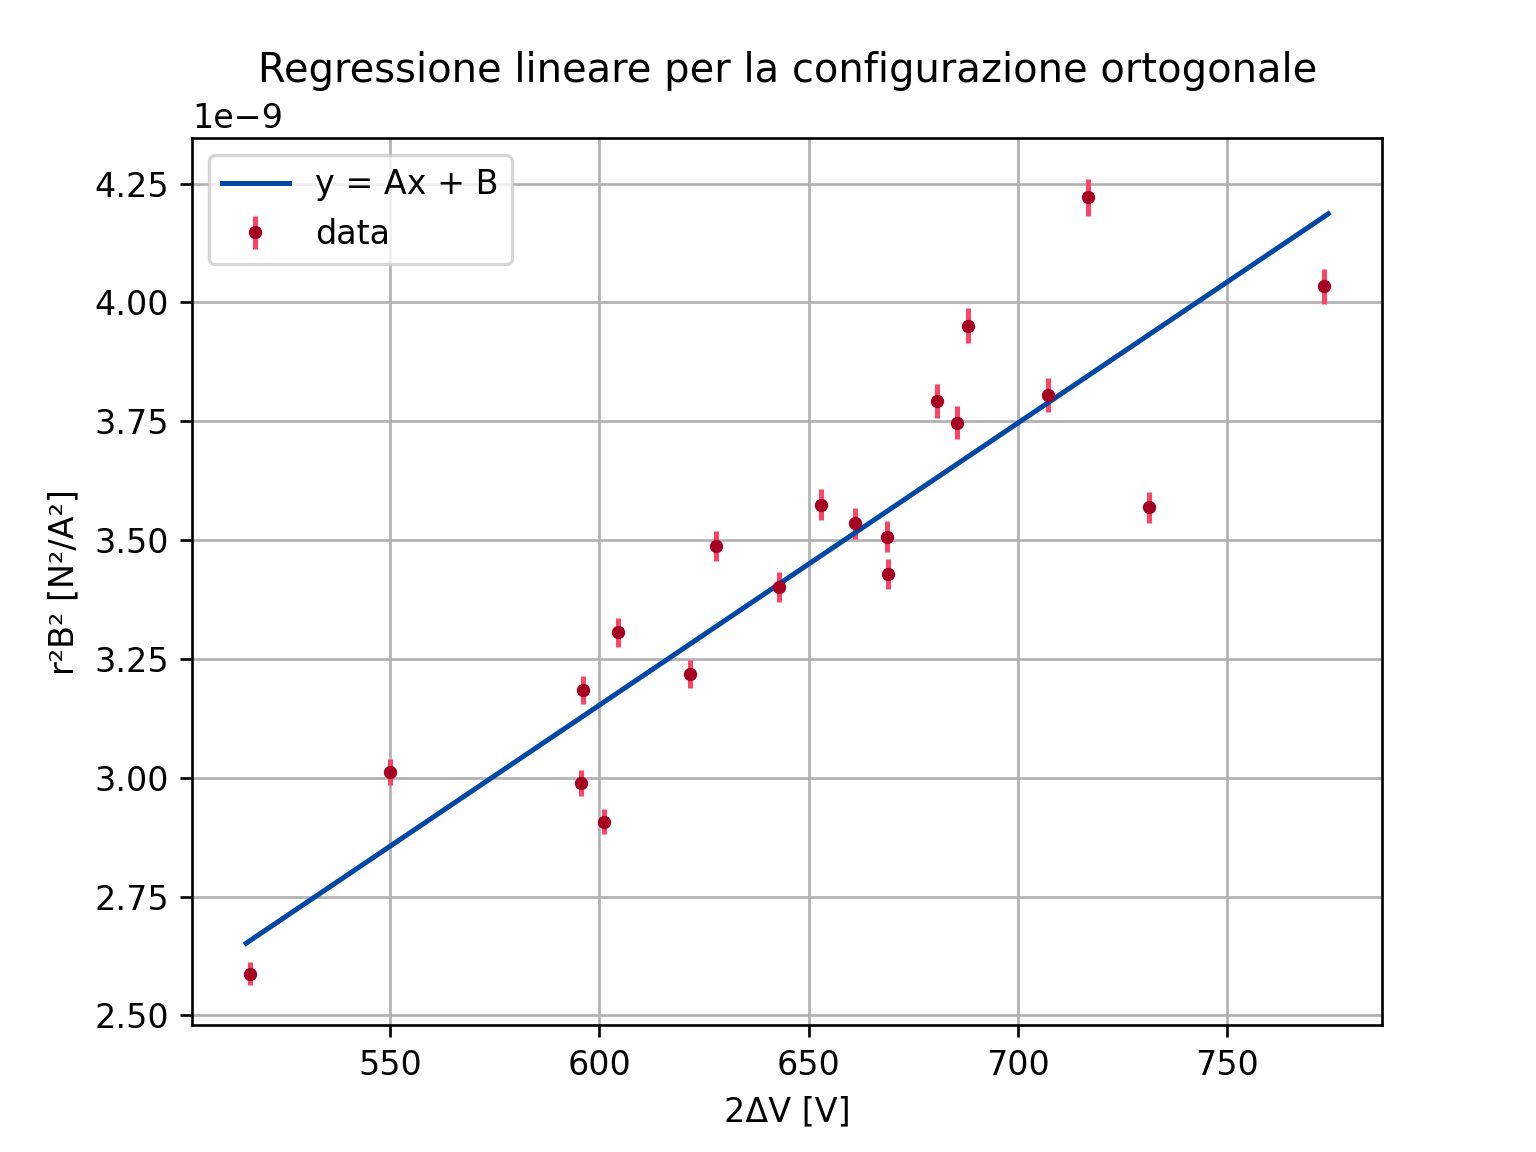
\includegraphics[width=0.70\textwidth]{plot/graph_ort.png}
    \caption{Regressione lineare relativa alla configurazione parallela, dove $A=(5.93 \pm 0.11) \cdot 10^{-12}\text{kg/C}$ e $B = (-4.08 \pm 0.72) \cdot 10^{-10} (\text{N/A})^2$.}
    \label{graph_ort}
\end{figure}

\begin{figure}[h]
    \centering
    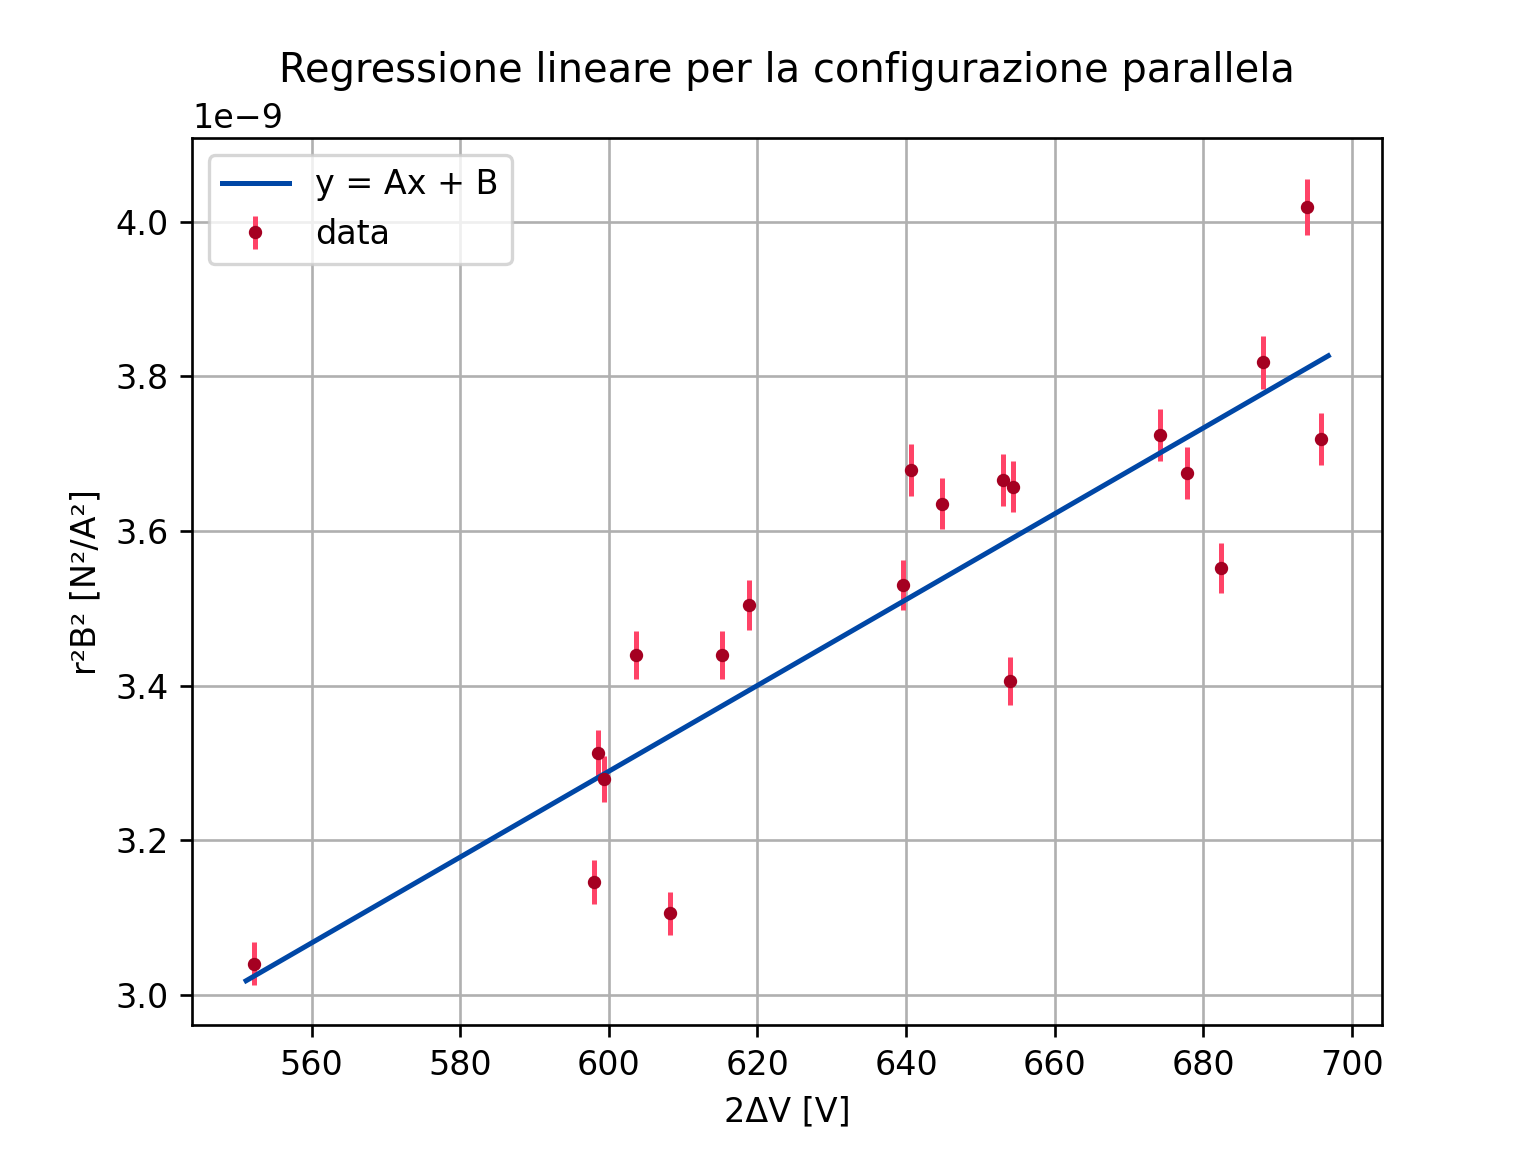
\includegraphics[width=0.70\textwidth]{plot/graph_par.png}
    \caption{Regressione lineare relativa alla configurazione parallela, dove $A=(5.44 \pm 0.18) \cdot 10^{-12}\text{kg/C}$ e $B = (-1.06 \pm 0.11) \cdot 10^{-10} (\text{N/A})^2$.}
    \label{graph_par}
\end{figure}

\begin{figure}[h]
    \centering
    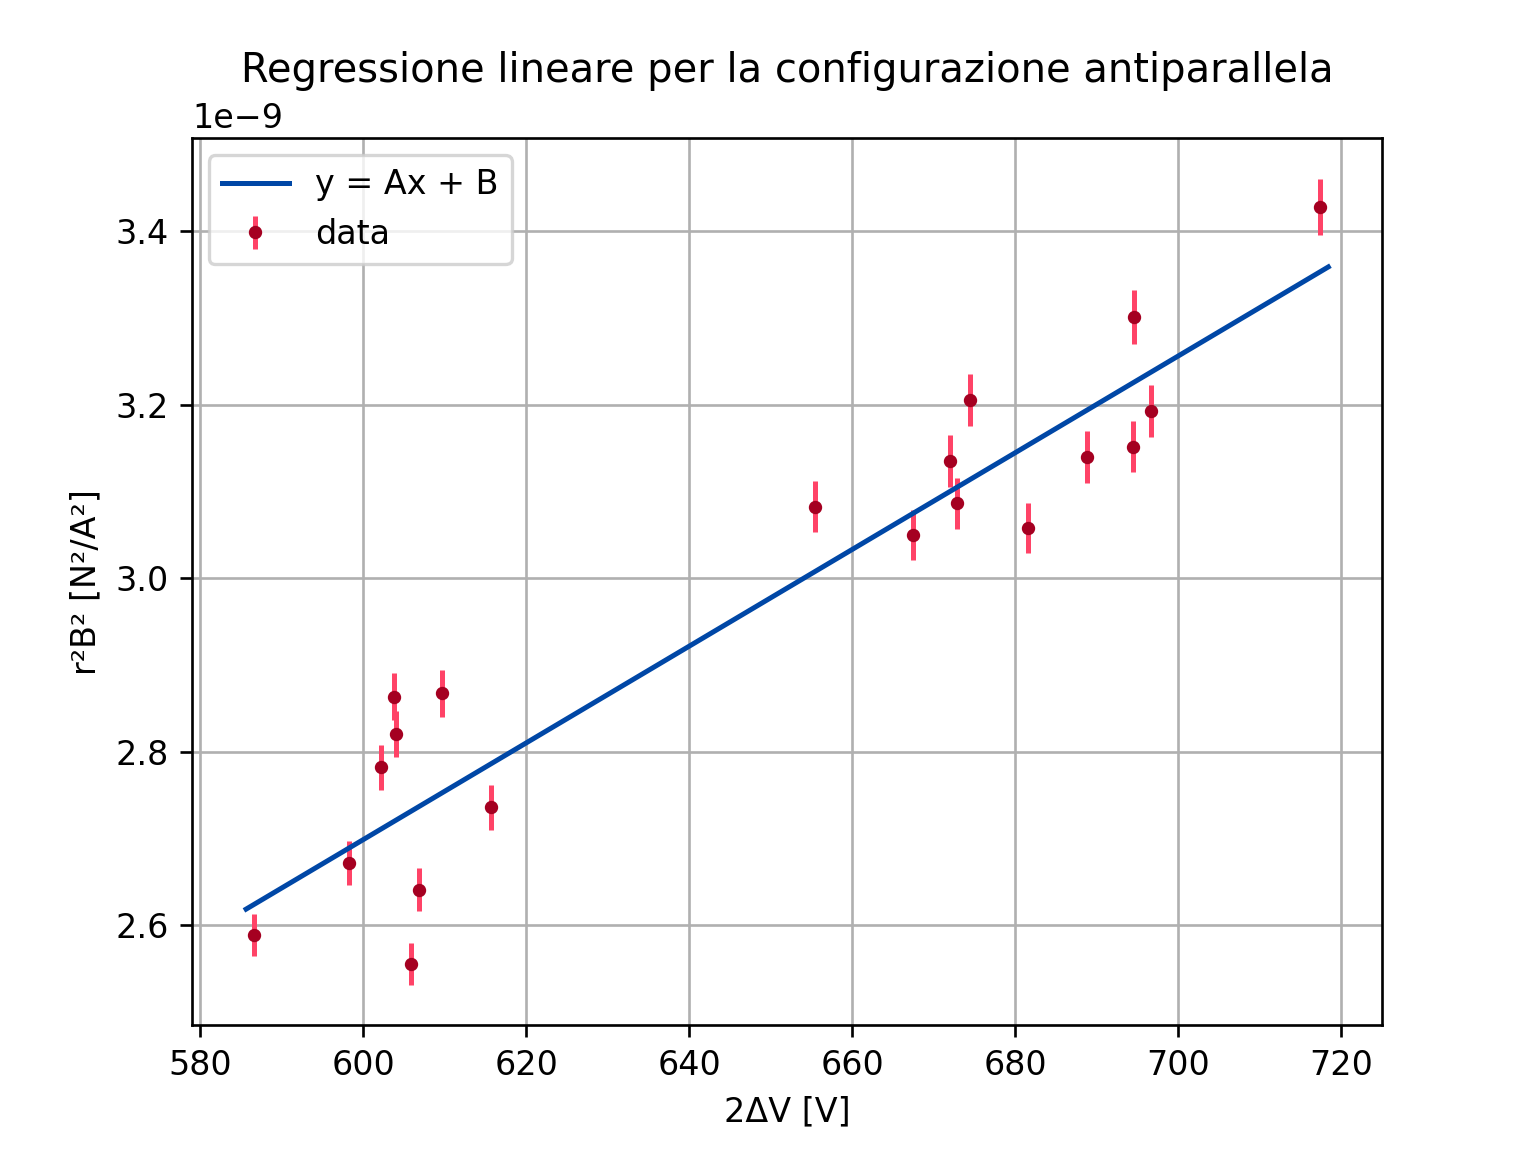
\includegraphics[width=0.70\textwidth]{plot/graph_apar.png}
    \caption{Regressione lineare relativa alla configurazione antiparallela, dove $A=(5.69 \pm 0.15) \cdot 10^{-12}\text{kg/C}$ e $B = (-5.95 \pm 0.99) \cdot 10^{-10} (\text{N/A})^2$.}
    \label{graph_par}
\end{figure}

\label{par:graph}

\end{document}